\chapter{Background}

\label{ch2_BACKGROUND}

%Replace \lipsum with text.
% You may have as many sections as you please. This is just for reference.

Video clips representing human actions can be classified based on features extracted from the video.
Object detection can add the object and people information to the recognition process.

This chapter explains three components in this project. 
Classifiers based on video features, object detectors and gives a brief introduction to Markov Logic Networks.

Classifiers based on video features use low level features like HoG-HoF features.
Using clustering of these features, each clip is represented in bag-of-features representation.
Finally, SVM is used to learn a model and classify the testing instances. Object detectors run on frames of videos and detect pre-defined objects along with
a confidence value for the detections. Such detections are useful to add object and people information
to the existing recognition system. Markov logic allows us to capture the semantic relationship using weighted first order formulae.
Thus use of Markov Logic makes the overall system robust towards noisy training data.


\section{Classification based on Video Features}
\label{section_STIP}
\subsection{Spatial Temporal Interest Points\index{Spatial Temporal Interest Points}}
As explained in \cite{laptev2005} spatial temporal interest points (\index{STIP}STIPs) are 3 dimensional points in 
space and time where the local video features show significant variations. 
In \cite{actionsInContext} the features extracted at STIPs are shown to perform satisfactorily for human activity recognition. 
At each STIP, \index{Histograms of Oriented Gradient}histograms of oriented gradient (HoG\index{HoG}) and \index{Histograms of Optical Flow} histograms of optical flow (\index{HoF}HoF) are evaluated.
The number of HoG and HoF features at each STIP are 72 and 90 respectively.
Concatenating vectors of HoG and HoF features, we get a single 162 element descriptor for each STIP. 

\subsection{Clustering}
After extraction of STIP features, each video clip roughly has $O(1000)$ such descriptors.
100,000 descriptors are sampled randomly from all the descriptors across all the clips.
While doing random sampling, each clip is given equal chance - this avoids biased sampling
towards ( or against) any particular class of videos if they happen to be longer ( or shorter) than other videos on an average.
These 100,000 random descriptors are clustered into $k = 200$ clusters using k-means.

\subsection{\index{Bag of Features Representation}Bag of Features Representation}
Each descriptor in each clip is clustered into one of the $k$ clusters using
least Euclidean distance. Thus each clip is represented by a $k$ sized vector
where $i^{th}$ element in this vector represents number of descriptors of that clip 
nearest to the $i^{th}$ cluster. This vector is called a Bag of Features (\index{BoF}BoF)
representation of the clip.

\begin{comment}
\begin{table}[t]
\centering
\begin{tabular}{| l | c |}
\hline
{\bf Activity Class} & {\bf Average Precision} \\ \hline
%
AnswerPhone & 11.36\% \\ \hline
DriveCar & 66.96\% \\ \hline
Eat & 45.45\% \\ \hline
FightPerson & 57.63\% \\ \hline
GetOutCar & 17.86\% \\ \hline
HandShake & 25.93\% \\ \hline
HugPerson & 15.15\% \\ \hline
Kiss & 18.18\% \\ \hline
Run & 38.78\% \\ \hline
SitDown & 40.96\% \\ \hline
SitUp & 5.26\% \\ \hline
StandUp & 35.20\% \\ \hline
Average AP & 31.56\% \\ \hline
%
\end{tabular}
\caption{Average precision for classification using only video features}
\label{table:AP_OnlyAction}
\end{table}
\end{comment}

\subsection{\index{Support Vector Machines}Support Vector Machines}
\label{AP_definition}
The BoF representation of all training clips are used to train a
support vector machine (\index{SVM}SVM) and BoF representation of a disjoint set of testing clips is classified using
learnt model. For training a SVM model, a radial basis function (RBF) kernel is used with parameters $C = 100$ 
and $\gamma = 0.01$. A one-versus-rest learning strategy is used to learn as many models as there are action classes.
In case of this data set, there are 12 action classes and thus 12 models are learnt.

Classification using only video features are compared taking \index{Average Average Precision|see {AAP}} average average precision as a measure.
As explained in \cite{actionsInContext}, average precision(AP) approximates area under recall-precision curve.
Thus, AP for each activity class is calculated and then finally averaged over all the classes, average AP (\index{AAP}AAP) is calculated.

\section{Object Detection}

\label{section_OBJ}

%Replace \lipsum with text.
% You may have as many sections as you please. This is just for reference.

Video clips of certain activity class have peculiar set of objects present in it.
If one could find objects present in the video clip, the activity prediction can 
potentially be made more confident. Below subsections introduce the object detection
method and its use in this project.

\subsection{Object Detector}
Object detector based on Discriminatively Trained Deformable Part Models \cite{voc-release4} was used in
the project. It can run on an image at a time. The detectors used in this project are trained on PASCAL 2007 data sets.
There are 20 models corresponding to 20 different objects.
These objects are : aeroplane, bicycle,
bird, boat, bottle, bus, car, cat, chair, cow, dining table, dog, horse,
motorbike, person, potted plant, sheep, sofa, train, tv monitor.
For this project only 10 relevant models were used : bicycle, bottle, bus, car,
chair, diningtable, motorbike, person, sofa, tvmonitor.

\subsection{Detection in Video}
Above described object detector models work on a single image at a time. To detect objects in video clips, 1 frame per second was extracted from the video clip and all the object detector models were run on the frame. In the data set used in this project, shortest clips is about 3-4 seconds long and longest clips are of the order of a minute. Frame rate is 24 frames per second.

The object detector models give a \index{Bounding Box}bounding box and a confidence (also called \index{Decision Value}decision value) for each detection 
on an absolute scale between $-\infty$ to $\infty$. 
Usually, a positive decision value represents true positive in all the models. 
A negative decision value represent lesser confident detection. 
It might be a true positive or a false positive. 
One can specify a threshold decision value before running object detector model 
so that only the detections at least as confident as the threshold are considered.
Usually, such thresholds are negative to allow detection of lesser confident objects also.

\subsection{Output of Object Detector}

The visual output of object detector looks as shown in figures \ref{fig:CarDetection} and \ref{fig:PersonDetection}. 
The red boxes are called as bounding boxes.
For each box, a confidence value is also evaluated - also called as decision value.

\floatstyle{plain}
\restylefloat{figure}
\begin{figure}[here]
\begin{center} 
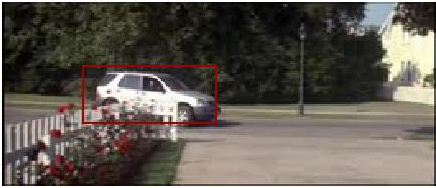
\includegraphics[scale=0.5]{car_detection_1.jpg} 
\caption{ Car detection in a frame. \label{fig:CarDetection}} 
\end{center} 
\end{figure}  

\begin{figure}[here]
\begin{center} 
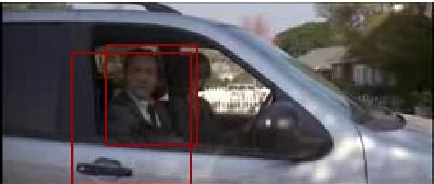
\includegraphics[scale=0.5]{person_detection_151.jpg} 
\caption{ Person detection in a frame. \label{fig:PersonDetection}} 
\end{center} 
\end{figure}  

\begin{comment}
\begin{table}[t,here]
\centering
\begin{tabular}{|l|c|}
\hline
\multicolumn{2}{|c|}{FRAME1} \\
\hline
 Car            &-0.181786\\
\hline
\multicolumn{1}{|c|}\vdots & \vdots \\
\hline
\multicolumn{1}{|c|}\vdots & \vdots \\
\hline
\multicolumn{2}{|c|}{FRAME151} \\
\hline
Person	&0.579786\\
\hline
Person	&-0.593087\\
\hline
\end{tabular}
\caption{Output of object detector with decision values}
\label{table:ObjDetection}
\end{table}
\end{comment}

\section{Markov Logic Networks}

\label{section_MLN}

%Replace \lipsum with text.
% You may have as many sections as you please. This is just for reference.

As explained in \cite{MarkovLogic}, Markov Logic consists of set of First order
logic (FOL) formulae associated with weights. The FOL formulae form the structure 
of Markov Logic Networks (MLNs). Background and theory of MLNs and calculation of
weights of formula is explained in the coming sections.

\subsection{Markov Networks}
\index{Markov Networks}Markov Network is an undirected graph $G$ with its nodes as set of variables $X = (X_1, X_2,\ldots, X_n) \in \rchi $.
Apart from graph, it also consists of \index{Potential Functions}potential functions $\phi_k$ for each clique $k$ in the graph.
Potential function $\phi_k$ is a real valued function of the state of $k^{th}$ clique.
The joint distribution is given by

\begin{equation}
	\label{jointDist}
	P(X = x) = \frac{1}{Z}{\displaystyle \prod_{k} \phi_{k}(x_{\{k\}})}
\end{equation}

where $x_{\{k\}}$ is the state of $k^{th}$ clique;
$Z$, also known as \index{Partition Function}partition function, is given by

\begin{equation}
	\label{partitionFunc}
	Z = \displaystyle \sum_{x \in \rchi} \displaystyle \prod_{k} \phi_k(x_{\{k\}}) 
\end{equation}

If clique potentials are replaced by exponentiation of weighted sum of features of state,
joint distribution can be given as

\begin{equation}
	\label{jointDistWeighted}
	P(X = x) = \frac{1}{Z} exp \left( \displaystyle \sum_i w_i f_i(x) \right)
\end{equation}

where $w_i$ is the weight of the $i^{th}$ clique and $f_i(x) \in \{0,1\}$ indicates state 
of the $i^{th}$ clique.

\subsection{Markov Logic}
The domain knowledge is captured by First Order Logic (FOL) formulae. In its basic form, 
first order knowledge base is a set of hard constraints over a set of possible worlds.
Because of these hard constraints, if a world does not satisfy even a single formula,
the world is considered as false or impossible.

Markov Logic uses FOL with soft constrains instead of hard. In markov logic, if a world
does not satisfy a formula $F_i$, it is considered as less probable world in comparison to a
world which satisfies $F_i$ assuming rest of the formulae have same state in both the worlds.

Definition \ref{MLNDef} from \cite{MarkovLogic} formally defines \index{Markov Logic Networks|see {MLN}}
Markov Logic Network (\index{MLN}MLN) as follows

\begin{defn}
	\label{MLNDef}
	A Markov Logic Network(MLN) L is a set of pairs $(F_i, w_i)$, where $F_i$ is a
	formula in first order logic and $w_i$ is weight associated with the formula - a real number.
	Together with a finite set of constants $C = \{c_1, c_2,\ldots,c_{|C|}\}$, MLN $L$
	defines a markov network, $M_{L,C}$ as follows :

	\begin{enumerate}
		\item $M_{L,C}$ contains one binary node for each possible grounding
			of each atom appearing in L. The value of the node is 1 if ground
			atom is true and 0 otherwise.
		\item $M_{L,C}$ contains one feature for each possible grounding of each
			formula $F_i$ in L. The value of the feature is 1 if the ground
			formula is true and 0 otherwise. The weight of the feature is
			$w_i$ associated with $F_i$ in L.
	\end{enumerate}
\end{defn}

Probability distribution over possible world $x$ specified by markov network $M_{L,C}$ is given by
\begin{equation}
	\label{jointDistMLN}
	P(X = x) = \frac{1}{Z} exp \left( \displaystyle \sum_{i = 1}^{F} w_i n_i(x)  \right)
\end{equation}
where $F$ is number of formulae in MLN and $n_i(x)$ is the number of true groundings of
$F_i$ in world $x$.
